\section{Numerical experiments}\label{sec:numerics}

\subsection{Setting}\label{sec:impl}
Real 2D FFTs in double precision; work is the number of forward plus inverse transforms, including conjugate-gradient work for Newton. Unless stated otherwise: $v^0=2\phi^n-\phi^{n-1}$; Armijo with $c=\frac14$, $\gamma=\frac12$, $\hat\omega_k=\min\{1,2\omega_{k-1}\}$; Newton--PCG (\cref{thm:newton}) with CG relative tolerance $10^{-2}$; \emph{practical} rule: \cref{alg:step} with $\eta=\frac12$, $c_R=1$ and the two-sided (T$_E$); \emph{tight} rule: $\nB{\Rn}\le10^{-10}$. A step is aborted (failure) if it exceeds its iteration cap ($300$ for gradient methods, $60$ for Newton unless stated) or $\nB{\Rn}>10^8$; a run diverges if an accepted iterate is non-finite or exceeds $10^3$ in $\nrm\cdot_\infty$. Norms: $\nrm\cdot$ discrete $L^2$; $\nrm\cdot_{-1}$; $\nrm{\gradN\cdot}$ the $H^1$ \emph{seminorm}; $\nrm\cdot_\infty$. Random data are uniform in $[-0.1,0.1]$ (NumPy default generator, stated seed) or band-limited (\cref{sec:num-seeds}). Simulation, diagnostics and plotting are separate scripts; every number below is extracted from saved data. In \cref{fig:robust,fig:estimator}: Newton--PCG blue circles, Armijo green squares, relaxed $\omega=\frac12$ orange triangles, linear $\omega=1$ purple diamonds; solid residual stopping, dashed fixed $K$; filled practical, open tight.

\subsection{Accuracy}\label{sec:num-accuracy}
Manufactured solution $\phi=\sin(2\pi x)\cos(2\pi y)\cos t$ on $(0,1)^2$ with forcing at $t_{n+1/2}$ (a linear term in $\Jn$, a constant in $\Rn$, a forcing term in \eqref{eq:identity}), $\phi^{-1}$ exact, $\eps=0.1$, $A=1$, $N=48$, $T=1$, $\tau=2^{-4},\dots,2^{-10}$; one wavenumber shell, and $\phi^3$ is resolved exactly at $N=48$, so the error is temporal. Error $e_j=\max_n\nrm{e^n}_{-1}$ at $\tau_j=2^{-j}$.

\begin{figure}[tbp]
\centering
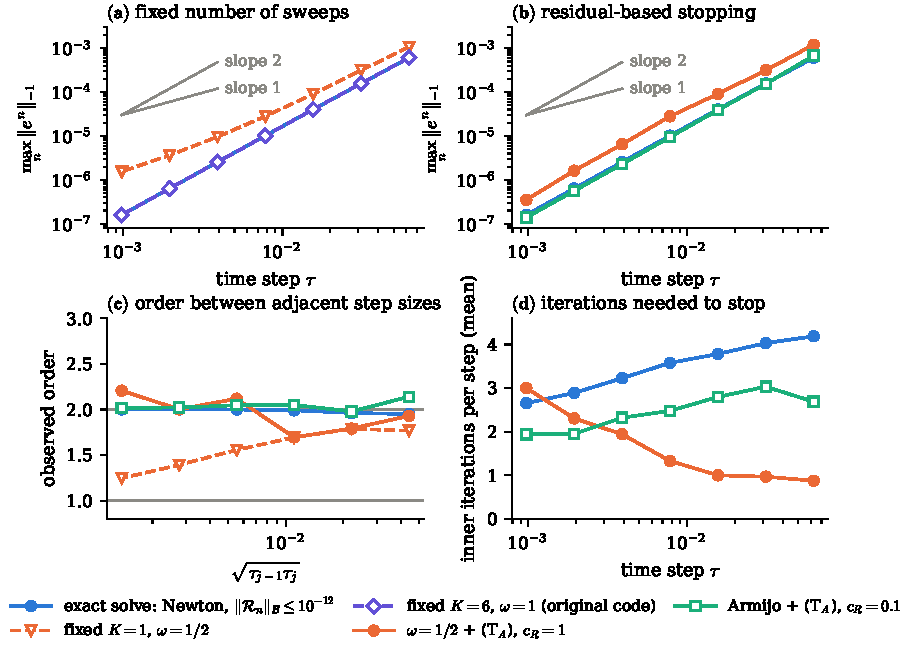
\includegraphics[width=\linewidth]{../figs/fig1_accuracy.pdf}
\caption{Accuracy (manufactured solution, $(0,1)^2$, $N=48$, $\eps=0.1$, $A=1$, $T=1$). (a,b)~$\max_n\nrm{e^n}_{-1}$ against $\tau$, fixed sweep counts (a) and residual-based stopping (b); exact solve (Newton, $\nB{\Rn}\le10^{-12}$) in both. (c)~$\log(e_{j-1}/e_j)/\log(\tau_{j-1}/\tau_j)$ at $\sqrt{\tau_{j-1}\tau_j}$. (d)~Mean inner iterations per step; values below one mean that the predictor passes (T$_A$) in some steps. All ten variants are in \cref{tab:accuracy}.}\label{fig:accuracy}
\end{figure}

\begin{table}[tbp]
\caption{Accuracy test, all inner-solve variants: observed orders $p_j$, error at $\tau_{10}=2^{-10}$ relative to the exact solve, and range over $\tau$ of the mean number of inner iterations per step.}\label{tab:accuracy}
\centering\scriptsize\setlength{\tabcolsep}{3.5pt}
\begin{tabular}{lcccccccc}
\toprule
& \multicolumn{6}{c}{$p_j=\log_2(e_{j-1}/e_j)$, $\tau_j=2^{-j}$} & $e_{10}/e^{\rm ex}_{10}$ & mean it.\\
\cmidrule(lr){2-7}
inner solve & $j=5$ & $j=6$ & $j=7$ & $j=8$ & $j=9$ & $j=10$ & & \\
\midrule
Newton, $\nB{\Rn}\le10^{-12}$ (exact) & 1.95 & 1.96 & 1.99 & 2.00 & 2.00 & 2.00 & 1.00 & 2.65--4.19\\
$\omega=1$, $K=1$ & 1.88 & 1.97 & 1.99 & 2.00 & 2.00 & 2.00 & 0.84 & 1.00--1.00\\
$\omega=1$, $K=2$ & 2.08 & 1.96 & 2.00 & 2.01 & 2.01 & 2.01 & 1.00 & 2.00--2.00\\
$\omega=1$, $K=6$ (original code) & 1.95 & 1.96 & 1.99 & 2.00 & 2.00 & 2.00 & 1.00 & 6.00--6.00\\
$\omega=\frac12$, $K=1$ & 1.77 & 1.79 & 1.69 & 1.56 & 1.39 & 1.25 & 9.68 & 1.00--1.00\\
$\omega=\frac12$, $K=2$ & 1.96 & 1.86 & 1.83 & 1.72 & 1.57 & 1.40 & 3.86 & 2.00--2.00\\
$\omega=\frac12$, $K=4$ & 1.95 & 1.94 & 1.95 & 1.92 & 1.85 & 1.73 & 1.56 & 4.00--4.00\\
$\omega=\frac12$ + (T$_A$), $c_R=1$ & 1.93 & 1.79 & 1.70 & 2.12 & 2.00 & 2.21 & 2.21 & 0.88--3.00\\
Armijo + (T$_A$), $c_R=1$ & 1.82 & 2.31 & 2.07 & 2.80 & 2.00 & 2.00 & 0.84 & 0.62--1.00\\
Armijo + (T$_A$), $c_R=0.1$ & 2.14 & 1.98 & 2.05 & 2.05 & 2.02 & 2.02 & 0.88 & 1.94--3.03\\
\bottomrule
\end{tabular}

\end{table}

\Cref{fig:accuracy,tab:accuracy} are consistent with \eqref{eq:fixedKres} and \cref{prop:linfixed}:
\begin{itemize}
\item $\omega=\frac12$, fixed $K=1,2,4$: $p_j$ decreases to $1.25,1.40,1.73$ at $j=10$; $e_{10}/e^{\rm ex}_{10}=9.7,3.9,1.6$.
\item $\omega=1$, fixed $K$: $p_j\in[1.88,2.08]$; $e_{10}/e^{\rm ex}_{10}=0.84,1.00,1.00$ for $K=1,2,6$ (leading term of \eqref{eq:fixedKres} vanishes).
\item $\omega=\frac12$ + (T$_A$): $p_j\in[1.70,2.21]$, $e_{10}/e^{\rm ex}_{10}=2.21$, $0.88$--$3.00$ iterations. Armijo + (T$_A$): $c_R=1$, $p_j\in[1.82,2.80]$; $c_R=0.1$, $p_j\in[1.98,2.14]$, ratio $0.88$--$1.12$ over $\tau$.
\item The isolated $p_8=2.80$ (Armijo, $c_R=1$) coincides with the change of the mean iteration count from $0.97$ to $1.00$; we attribute it to the switch between accepting the predictor and one iteration.
\end{itemize}
Spatial accuracy ($\phi=0.4\cos t\sin(2\pi x)e^{\cos(2\pi y)}$, $\tau=10^{-4}$, $T=0.01$, exact solves): discrete $L^2$ errors $4.0\cdot10^{-3}$, $2.6\cdot10^{-5}$, $2.4\cdot10^{-7}$, $3.5\cdot10^{-9}$ for $N=8,12,16,20$, and $2.8\cdot10^{-9}$ for $24\le N\le64$ (an $N$-independent floor, attributed to the time discretization).

\subsection{Robustness and cost}\label{sec:num-robust}
\emph{One hard step} (\cref{fig:robust}(a,b)): step $n=20$ ($t=0.08$, end of the spinodal stage, $\max|\phi^n|\approx1.05$) of the problem $[0,6.4)^2$, $N=256$, $\eps=0.02$, $\tau=0.004$, seed~$1$; common history from Newton; runs to $\nB{\Rn}\le10^{-12}$ or $150$ iterations. Transforms to acceptance (practical / tight $10^{-10}$):

\smallskip
\centerline{\small\begin{tabular}{lcccc}
\toprule
& linear $\omega=1$ & relaxed $\omega=\frac12$ & Armijo & Newton--PCG\\
\midrule
$A=0$, $\theta_N=1.83$ & diverges ($\nB{\Rn}:0.20\to3\cdot10^{17}$) & 53 / 149 & 31 / 69 & 35 / 59\\
$A=2$, $\theta_N=0.39$ & 115 / 255 & 33 / 65 & 25 / 47 & 27 / 43\\
\bottomrule
\end{tabular}}
\smallskip

\noindent\emph{Whole runs} (\cref{tab:solver}, $T=1$): the unrelaxed iteration diverges in $4$ of $6$ settings. \Cref{cor:linear} guarantees convergence if $M_0<(2/(3\theta_N))^{1/2}=0.85,0.60,0.43$ ($A=0$) and $1.44,1.30,1.23$ ($A=2$) for $\tau=0.001,0.004,0.016$; the divergent runs fail after the amplitude exceeds these values (the condition is sufficient, not necessary). $\omega=\frac12$ fails only for $A=0$, $\tau=0.016$, where $\frac12>2/(1+q_0)$ as soon as $M_0>0.74$. Armijo and Newton converge in all settings.

\begin{figure}[tbp]
\centering
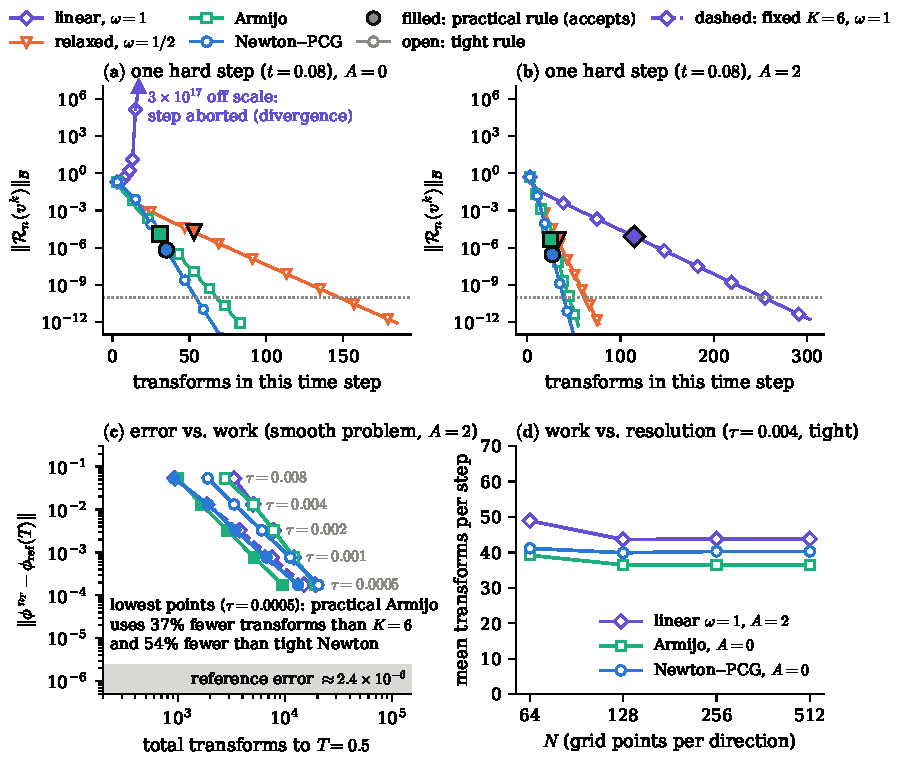
\includegraphics[width=\linewidth]{../figs/fig2_robustness.pdf}
\caption{Robustness and cost. (a,b)~$\nB{\Rn(v^k)}$ against cumulative transforms in step $n=20$ ($t=0.08$) of $[0,6.4)^2$, $N=256$, $\eps=0.02$, $\tau=0.004$, seed~$1$; large filled markers: practical acceptance; dotted line: $10^{-10}$. In (a) the last residual of the unrelaxed iteration, $3\cdot10^{17}$, lies above the range (triangle); the step is then aborted. (c)~Discrete $L^2$ error at $T=0.5$ against total transforms for the smooth interface problem ($[0,2)^2$, $N=128$, $\eps=0.04$, $A=2$, $\tau=0.008,\dots,0.0005$), reference $\tau=6.25\cdot10^{-5}$, Newton to $10^{-12}$; shaded: below the Richardson estimate $2.4\cdot10^{-6}$ of the reference error; annotation: savings at the smallest $\tau$ from the unrounded counts ($9444$ against $15000$ and $20412$). (d)~Mean transforms per step against $N$ ($[0,6.4)^2$, $\eps=0.04$, $\tau=0.004$, $T=1$, tight rule, modes $|k_i|\le16$).}\label{fig:robust}
\end{figure}

\begin{table}[tbp]
\caption{$[0,6.4)^2$, $N=256$, $\eps=0.02$, seed~$1$, $T=1$: mean inner iterations (it) and transforms (FFT) per step; ``div.'' divergence. $\theta_N=0.91,1.83,3.65$ ($A=0$), $0.32,0.39,0.44$ ($A=2$) for $\tau=0.001,0.004,0.016$.}\label{tab:solver}
\centering\scriptsize\setlength{\tabcolsep}{3pt}
\begin{tabular}{llrrrrrrrrrrrr}
\toprule
& & \multicolumn{4}{c}{$\tau=0.001$} & \multicolumn{4}{c}{$\tau=0.004$} & \multicolumn{4}{c}{$\tau=0.016$}\\
\cmidrule(lr){3-6}\cmidrule(lr){7-10}\cmidrule(lr){11-14}
& & \multicolumn{2}{c}{$A=0$} & \multicolumn{2}{c}{$A=2$} & \multicolumn{2}{c}{$A=0$} & \multicolumn{2}{c}{$A=2$} & \multicolumn{2}{c}{$A=0$} & \multicolumn{2}{c}{$A=2$}\\
stop & method & it & FFT & it & FFT & it & FFT & it & FFT & it & FFT & it & FFT\\
\midrule
\multirow{4}{*}{\shortstack[l]{$\nB{\Rn}\le10^{-10}$}} & linear, $\omega=1$ & \multicolumn{2}{c}{div.} & 18.8 & 41 & \multicolumn{2}{c}{div.} & 41.0 & 85 & \multicolumn{2}{c}{div.} & \multicolumn{2}{c}{div.}\\
 & relaxed, $\omega=\frac12$ & 22.4 & 48 & 23.1 & 49 & 83.7 & 170 & 26.8 & 57 & \multicolumn{2}{c}{div.} & 30.2 & 63\\
 & Armijo & 15.0 & 33 & 18.8 & 41 & 28.1 & 59 & 18.6 & 40 & 57.2 & 117 & 19.8 & 43\\
 & Newton--PCG & 3.4 & 36 & 3.2 & 27 & 4.4 & 54 & 4.0 & 34 & 5.5 & 81 & 4.8 & 41\\
\midrule
\multirow{4}{*}{\shortstack[l]{(T$_E$)+(T$_A$)}} & linear, $\omega=1$ & \multicolumn{2}{c}{div.} & 8.2 & 19 & \multicolumn{2}{c}{div.} & 16.0 & 35 & \multicolumn{2}{c}{div.} & \multicolumn{2}{c}{div.}\\
 & relaxed, $\omega=\frac12$ & 11.1 & 25 & 11.7 & 26 & 21.6 & 46 & 11.2 & 25 & \multicolumn{2}{c}{div.} & 10.5 & 24\\
 & Armijo & 7.2 & 17 & 8.2 & 19 & 10.5 & 24 & 8.1 & 19 & 17.2 & 37 & 7.2 & 17\\
 & Newton--PCG & 2.0 & 22 & 2.1 & 18 & 2.2 & 27 & 2.2 & 20 & 2.6 & 39 & 2.3 & 22\\
\bottomrule
\end{tabular}

\end{table}

\noindent\emph{Work at measured accuracy} (\cref{fig:robust}(c)). The random problem is unsuitable: halving $\tau$ changes it by $O(1)$ (\cref{sec:num-bench}), reflecting $e^{CT\eps^{-2}}$ in \cref{thm:error}. We use, on $[0,2)^2$ with $L=2$,
\[
\phi^0=\tanh\frac{\max\{d_\star,d_1,d_2\}}{\sqrt2\eps},\qquad d_\star=0.22L+0.04L\cos6\vartheta-r,\qquad d_i=0.11L-|x-c_i|,
\]
with polar coordinates $(r,\vartheta)$ about $(0.32L,0.5L)$ (a six-lobed star), $c_1=(0.7L,0.36L)$, $c_2=(0.7L,0.64L)$; the circles merge and the star relaxes; $\nrm{\phi_{\rm ref}(T)}=1.87$. All six variants have the same error at each $\tau$ (spread $<0.05\%$), with order $2.01$--$2.13$, and none fails. Transforms relative to the original code ($\omega=1$, $K=6$): practical Armijo $1.08,0.88,0.77,0.69,0.63$ for $\tau=0.008,\dots,0.0005$; practical Newton $0.88$--$1.02$; tight variants $1.27$--$3.58$. Against the same method run to the tight tolerance, the practical rule uses $50.5$--$67.3\%$ (Armijo) and $35.4$--$51.5\%$ (Newton) fewer transforms. The original code is as accurate here ($A=2$, smooth data) but diverges for $A=0$ (panel (a)).

\noindent\emph{Mesh} (\cref{fig:robust}(d)): from $N=64$ to $512$ the transforms per step change $49\to44$ (linear, $A=2$), $39\to36$ (Armijo, $A=0$), $41\to40$ (Newton, $A=0$), consistent with the $N$-independence of $\theta_N$ in \cref{thm:local,thm:newton}.

\subsection{Reliability of the a posteriori bound}\label{sec:num-estimator}
$[0,3.2)^2$, $N=128$, $\eps=0.02$, $A=2$, $\tau=0.004$, seed~$3$; reference step solutions by Newton to $\nB{\Rn}\le10^{-13}$. (a) $739$ iterates (first $15$ of $\omega=1$ and $\omega=\frac12$ at $n=0,10,\dots,240$): $\nBi{v-\phi^{n+1}}/\nB{\Rn(v)}\in[0.589,0.9996]$ ($\omega=1$: $\ge0.589$; $\omega=\frac12$: $\ge0.654$), against the guaranteed interval $[1/(1+q_{\max}),1]=[0.448,1]$ of \eqref{eq:apost} with $q_{\max}=1.23$. (b) First iterate with $\nB{\Rn}\le\mathrm{tol}$, $\mathrm{tol}=10^{-2},\dots,10^{-10}$, four methods, $n=5,15,\dots,245$: $500$ accepted iterates, error/tol $\in[2.2\cdot10^{-3},0.974]$, no violation.

\begin{figure}[tbp]
\centering
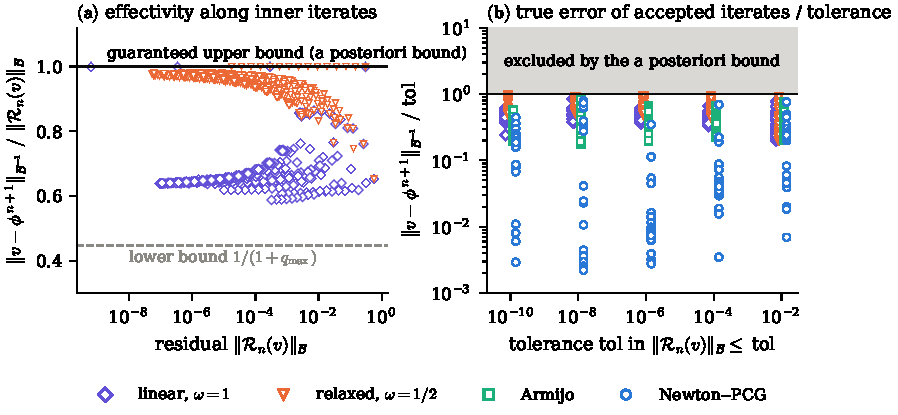
\includegraphics[width=\linewidth]{../figs/fig3_estimator.pdf}
\caption{A posteriori bound ($[0,3.2)^2$, $N=128$, $\eps=0.02$, $A=2$, $\tau=0.004$, seed~$3$; references by Newton to $10^{-13}$). (a)~$\nBi{v-\phi^{n+1}}/\nB{\Rn(v)}$ for $739$ iterates; dashed: $1/(1+q_{\max})$ with $q_{\max}=\max q(M_v)$, $M_v$ as in \cref{thm:apost}, $\theta_N=0.39$. (b)~True error/tolerance for the first accepted iterate ($500$ iterates, methods offset horizontally); the shaded region is excluded by \cref{thm:apost}.}\label{fig:estimator}
\end{figure}

\subsection{Coarsening benchmark}\label{sec:num-bench}
The problem of \cite{ChengWangWiseYue2016}: $[0,12.8)^2$, $N=512$, $\eps=0.02$, $A=0$, $\tau=0.004$, $T=10$, seed~$1$ (mean $-8.7\cdot10^{-5}$); practical and tight solvers in lockstep, i.e.\ two solvers of the \emph{same} fully discrete problem. The trajectory is not converged in time: the fastest linear mode has rate $\lambda_{\max}=(4\eps^2)^{-1}=625$, $\tau\lambda_{\max}=2.5$, and halving $\tau$ changes the solution by $8.7$ ($t=0.2$) and $12.2$ ($t=1$) in $L^2$; the energies $E+|\Omega|/4$ of the $\tau$ and $\tau/2$ runs differ by $0.4\%$ and $0.8\%$.

\begin{figure}[tbp]
\centering
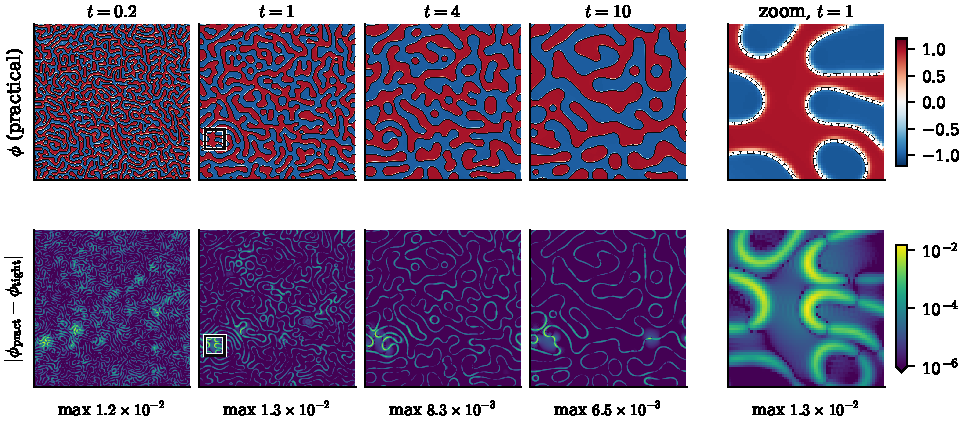
\includegraphics[width=\linewidth]{../figs/fig4_coarsening.pdf}
\caption{Coarsening benchmark ($[0,12.8)^2$, $N=512$, $\eps=0.02$, $A=0$, $\tau=0.004$, seed~$1$); both solvers solve the same discrete problem, which is not converged in $\tau$. Columns 1--4: full domain at $t=0.2,1,4,10$; column 5: the $1.6\times1.6$ box ($64^2$ points) marked at $t=1$, centred on the largest difference. Top: practical $\phi$, limits $[-1.2,1.2]$ (all values in $[-1.149,1.040]$); black: tight zero level set; white dashed (column 5): practical zero level set. Bottom: $|\phi_{\rm pract}-\phi_{\rm tight}|$ on $[10^{-6},1.5\cdot10^{-2}]$ (contains every maximum, stated beneath).}\label{fig:coarsening}
\end{figure}

\begin{figure}[tbp]
\centering
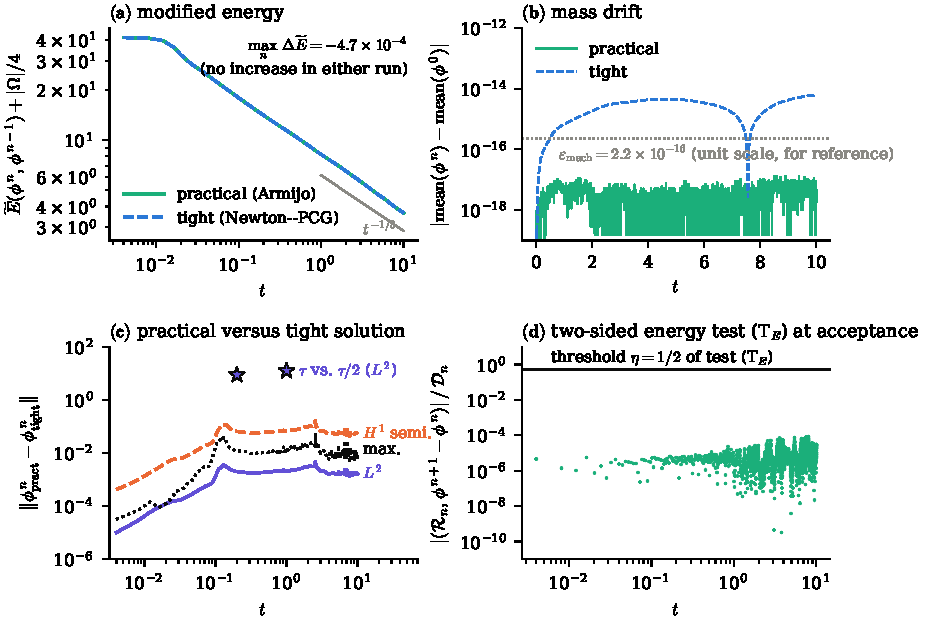
\includegraphics[width=\linewidth]{../figs/fig5_structure.pdf}
\caption{Structure on the benchmark of \cref{fig:coarsening}; practical solid (green), tight dashed (blue). (a)~$\Et(\phi^n,\phi^{n-1})+|\Omega|/4$; grey: slope $-\frac13$. (b)~$|\mean(\phi^n)-\mean(\phi^0)|$; dotted: machine epsilon $2.2\cdot10^{-16}$ as a unit-scale reference, not a bound. (c)~Practical minus tight in $L^2$, $H^1$ seminorm and maximum norm; stars: $L^2$ difference of tight solutions with $\tau$ and $\tau/2$. (d)~$|\ip{\Rn(v)}{v-\phi^n}|/\Dn(v)$ at acceptance; the two-sided test requires $\le\eta=\frac12$ and is stronger than needed for decay (\cref{rem:onesided}).}\label{fig:structure}
\end{figure}

Practical: $7.3$ iterations per step (max $18$), $17.6$ transforms; tight: $3.6$ Newton iterations (max $6$), $45.0$ transforms; all steps accepted with $\nrm{\rho^n}\le1.6\cdot10^{-5}=c_R\tau^2$. Differences (\cref{fig:coarsening,fig:structure}): snapshot median $\le1.5\cdot10^{-6}$, 99th percentile $\le2.2\cdot10^{-4}$, maximum $\le1.35\cdot10^{-2}$; over the run $\max_n\nrm{\phi_{\rm p}^n-\phi_{\rm t}^n}=4.7\cdot10^{-3}$ ($t\approx2.5$; relative $\le4\cdot10^{-4}$ since $\nrm{\phi}\in[11.0,12.4]$), $H^1$ seminorm $<0.16$, maximum norm $<0.05$. $\Et$ decreases at every step of both runs (largest change $-4.7\cdot10^{-4}$; relative difference of $\Et+|\Omega|/4$ between runs $\le1.7\cdot10^{-5}$); between $t=1$ and $10$, $\Et+|\Omega|/4\sim t^{-0.36}$, close to $t^{-1/3}$ \cite{KohnOtto2002}. Maximal mass drift $1.3\cdot10^{-17}$ (practical) and $6.0\cdot10^{-15}$ (tight). (T$_E$) ratio $\le7.9\cdot10^{-5}$ (median $6\cdot10^{-6}$).

\subsection{Interface evolution: merger and Ostwald ripening}\label{sec:num-interface}
Protocol: (1) tight solutions for $\tau=8\tau_0,\dots,\tau_0$ ($\tau_0=2.5\cdot10^{-4}$ star, $5\cdot10^{-4}$ droplets); (2) $N$ against $2N$; (3) the reported observables; (4) practical and tight solvers in lockstep at the production resolution, same data and output times, constant $\tau$. Observables (\cref{app:observables}): the number of components of $\{\phi>0\}$ (periodic, 4-connectivity), a merger time being its first decrease; the interface-displacement proxy $\delta_\Gamma(a,b)=\nrm{a-b}_{L^1}/(2|\Gamma_b|)$, which equals the mean normal displacement to leading order for equal profiles and nearby interfaces but is not a geometric measurement or bound in general; the equivalent radius $R_j=(\mathcal A_j/\pi)^{1/2}$ from the marching-squares zero contour nearest to droplet $j$'s previous centroid (within $0.15$), a disappearance time being the first step without such a contour.

\begin{table}[tbp]
\caption{Resolution study (tight solver). Star: $\delta_\Gamma$ against $N=128$, $\tau=2.5\cdot10^{-4}$ at $t=0.1,0.25,0.5$, and merger times. Droplets: largest difference of the radii at $t=0.15,1,2$ against the run in column~3, and disappearance times $t_1,t_2$. Production resolutions~$^\ast$.}\label{tab:resolution}
\centering\scriptsize\setlength{\tabcolsep}{4pt}
\begin{tabular}{lllcccc}
\toprule
\multicolumn{7}{l}{\emph{Star and two circles} ($A=2$, $T=0.5$): displacement proxy $\delta_\Gamma(t)$ against $N=128$, $\tau=2.5\cdot10^{-4}$}\\
$N$ & $\tau$ & & $\delta_\Gamma(0.1)$ & $\delta_\Gamma(0.25)$ & $\delta_\Gamma(0.5)$ & $t_{m,1}$, $t_{m,2}$\\
\midrule
128 & $0.002$ &  & $8.0\cdot10^{-4}$ & $1.5\cdot10^{-3}$ & $3.3\cdot10^{-4}$ & $0.03400$, $0.1980$\\
128 & $0.001$ & $^\ast$ & $1.9\cdot10^{-4}$ & $3.4\cdot10^{-4}$ & $7.5\cdot10^{-5}$ & $0.03000$, $0.1940$\\
128 & $0.0005$ &  & $3.7\cdot10^{-5}$ & $6.6\cdot10^{-5}$ & $1.4\cdot10^{-5}$ & $0.02900$, $0.1935$\\
128 & $0.00025$ & ref. & -- & -- & -- & $0.02875$, $0.1930$\\
256 & $0.00025$ &  & $3.1\cdot10^{-5}$ & $3.4\cdot10^{-5}$ & $1.6\cdot10^{-5}$ & $0.02850$, $0.1930$\\
\midrule
\multicolumn{7}{l}{\emph{Unequal droplets} ($A=0$, $T=2$): radii at $t=0.15,1,2$ against the run in column 3}\\
$N$ & $\tau$ & against & \multicolumn{3}{c}{$\max_{j,k}|R_j(t_k)-R_j^{\rm cmp}(t_k)|$} & $t_1$, $t_2$\\
\midrule
256 & $0.004$ & $N=256$, $\tau=0.001$ & \multicolumn{3}{c}{$1.3\cdot10^{-3}$} & $0.2040$, $1.5560$\\
256 & $0.002$ & $N=256$, $\tau=0.001$ & \multicolumn{3}{c}{$5.3\cdot10^{-5}$} & $0.2000$, $1.5540$\\
256 & $0.001$ & $^\ast$ & \multicolumn{3}{c}{--} & $0.1990$, $1.5520$\\
256 & $0.0005$ & $N=256$, $\tau=0.001$ & \multicolumn{3}{c}{$1.3\cdot10^{-5}$} & $0.1985$, $1.5520$\\
128 & $0.0005$ & $N=256$, $\tau=0.0005$ & \multicolumn{3}{c}{$1.7\cdot10^{-4}$} & $0.1985$, $1.5520$\\
512 & $0.001$ & $N=256$, $\tau=0.001$ & \multicolumn{3}{c}{$4.2\cdot10^{-5}$} & $0.1990$, $1.5520$\\
\bottomrule
\end{tabular}

\end{table}

\emph{Merger} (\cref{fig:star}): the problem of \cref{fig:robust}(c), $[0,2)^2$, $\eps=0.04$, $A=2$, $T=0.5$; the circles merge at $t\approx0.029$, the relaxed star joins them through a neck at $t\approx0.193$. \Cref{tab:resolution}: $\delta_\Gamma$ decreases at second order in $\tau$; at $N=128$, $\tau=10^{-3}$, $\delta_\Gamma\le3.4\cdot10^{-4}\approx h/46$ and the merger times differ from the reference by $1.25\tau$ and $\tau$; $2N$ gives $\delta_\Gamma\le3.4\cdot10^{-5}$. Practical versus tight: identical merger steps ($0.030$, $0.194$); $\delta_\Gamma\le8.3\cdot10^{-8}$ at the output times against $6.1\cdot10^{-5}$--$2.8\cdot10^{-4}$ for $\tau$ versus $\tau/2$ (a factor $700$--$4600$ in $\delta_\Gamma$); fields differ by $\le8.8\cdot10^{-7}$ in $L^2$ and $\le6.1\cdot10^{-6}$ pointwise, largest at the neck; $5140$ transforms (practical Armijo) against $11180$ (tight Newton--PCG), $54.0\%$ fewer. Cost peaks in the first steps and around the second merger, briefly for the tight solver ($t\approx0.19$--$0.24$), longer for the practical one ($t\approx0.17$--$0.33$).

\begin{figure}[tbp]
\centering
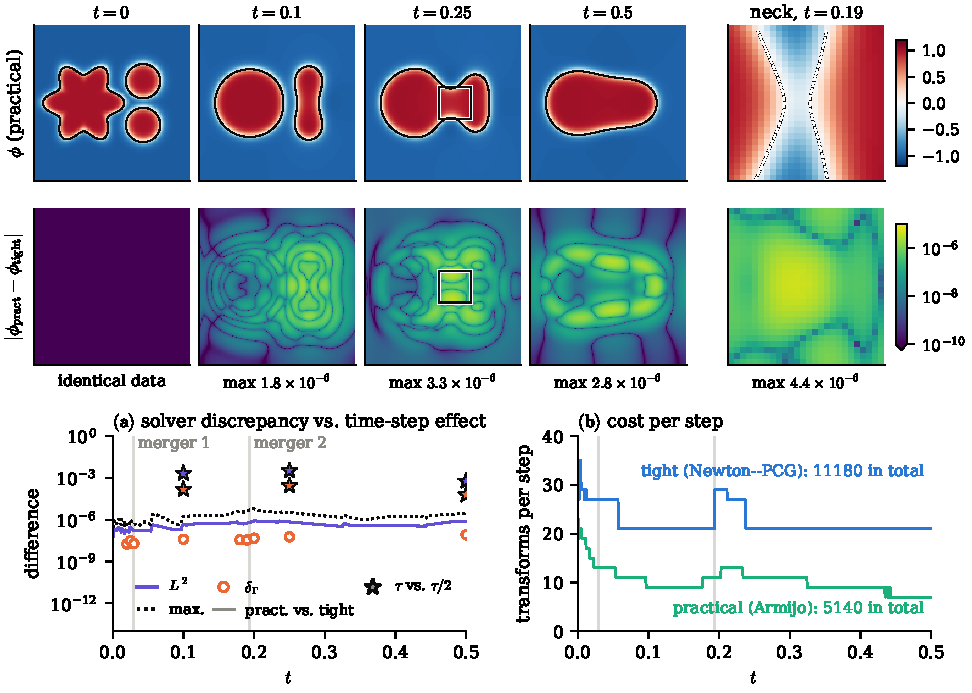
\includegraphics[width=\linewidth]{../figs/fig6_star.pdf}
\caption{Merger ($[0,2)^2$, $N=128$, $\eps=0.04$, $A=2$, $\tau=10^{-3}$). Top: practical $\phi$ at $t=0,0.1,0.25,0.5$, limits $[-1.2,1.2]$ (values in $[-1.019,1.044]$), tight zero level set black; column~5: the box marked at $t=0.25$ ($0.41^2$, $26^2$ points) at $t=0.19$, practical zero level set white dashed. Bottom: $|\phi_{\rm pract}-\phi_{\rm tight}|$ on $[10^{-10},10^{-5}]$ (contains every maximum). (a)~Practical minus tight: $L^2$ (line), maximum norm (dotted), $\delta_\Gamma$ (circles); stars: the same $L^2$ and $\delta_\Gamma$ for tight $\tau=10^{-3}$ against $5\cdot10^{-4}$; vertical lines: merger times. (b)~Transforms per step.}\label{fig:star}
\end{figure}

\emph{Ostwald ripening} (\cref{fig:droplets}): $[0,2)^2$, $\eps=0.04$, $A=0$, droplets ($\phi=1$ inside) of radii $0.16,0.24,0.32$ centred at $(1.00,1.50)$, $(1.45,0.72)$, $(0.58,0.62)$, tanh profiles of the periodic distance, closest interfaces $0.32\approx8\eps$ apart. The smallest droplet disappears at $t\approx0.199$, the middle one at $t\approx1.552$, and $R_3(2)=0.4195$. At $N=256$, $\tau=10^{-3}$ the radii at $t=0.15,1,2$ agree with $\tau/2$ to $1.3\cdot10^{-5}$ and with $N=512$ to $4.2\cdot10^{-5}$; disappearance times agree within one step. Practical versus tight: identical disappearance steps; median $|R_j^{\rm p}-R_j^{\rm t}|\le2.4\cdot10^{-7}$ against a median time-step effect $\ge1.5\cdot10^{-6}$; maximum $7.4\cdot10^{-5}$ ($R_2$, $t=1.551$) against a time-step effect of $2.2\cdot10^{-3}$ there; $\delta_\Gamma\le3.4\cdot10^{-7}$ at the output times; $\le4.3\cdot10^{-5}$ in $L^2$ over the run; $14492$ transforms (practical Armijo) against $43278$ (tight Newton--PCG), $66.5\%$ fewer.

\begin{figure}[tbp]
\centering
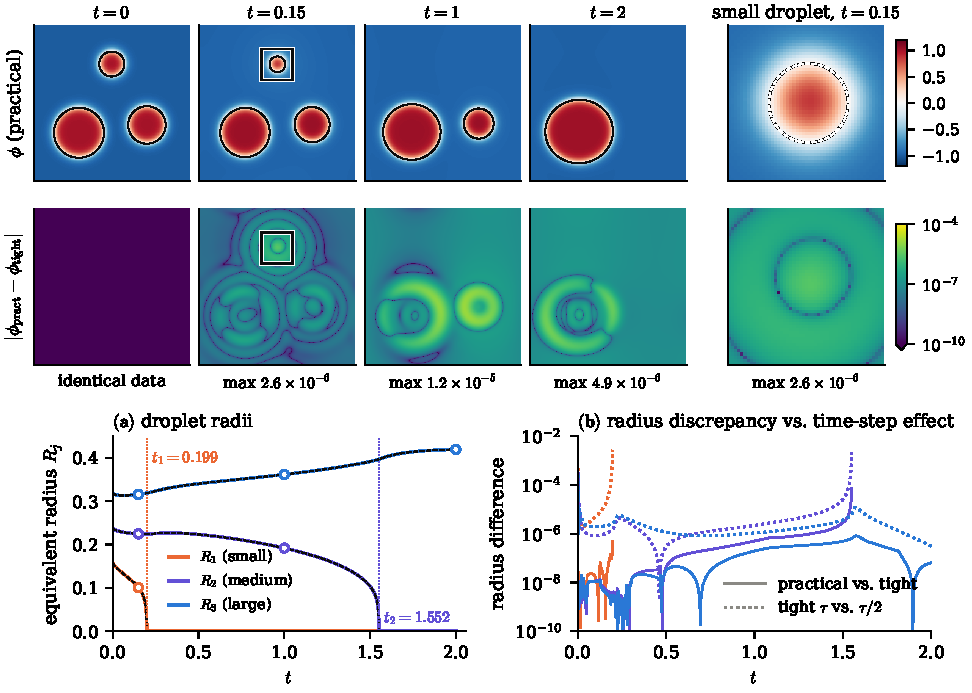
\includegraphics[width=\linewidth]{../figs/fig7_droplets.pdf}
\caption{Ostwald ripening ($[0,2)^2$, $N=256$, $\eps=0.04$, $A=0$, $\tau=10^{-3}$). Top: practical $\phi$ at $t=0,0.15,1,2$, limits $[-1.2,1.2]$ (values in $[-1.000,1.041]$), tight zero level set black; column~5: the small droplet at $t=0.15$ (box $0.40^2$, $51^2$ points), practical zero level set white dashed. Bottom: $|\phi_{\rm pract}-\phi_{\rm tight}|$ on $[10^{-10},10^{-4}]$. (a)~$R_j(t)$: practical (coloured), tight (black dashed), tight with $\tau/2$ at the output times (circles); dotted: disappearance times (identical in both runs). (b)~$|R_j^{\rm p}-R_j^{\rm t}|$ (solid) and $|R_j(\tau)-R_j(\tau/2)|$ of the tight solver (dotted); colours as in (a).}\label{fig:droplets}
\end{figure}

\subsection{Nonzero mean, three seeds}\label{sec:num-seeds}
$[0,6.4)^2$, $N=256$, $\eps=0.04$, $A=0$, $\tau=0.002$, $T=5$, $\phi^0=\bar\phi+0.05\,P/\max|P|$ with $\bar\phi=-0.5$ and $P(x)=\sum_{|k_1|,|k_2|\le24}c_ke^{\mathrm i\kappa_k\cdot x}$, $\hat P_0=c_0=0$, $c_{-k}=\overline{c_k}$ (so $P$ is real), $c_k=\frac12(z_k+\overline{z_{-k}})$ with $\mathrm{Re}\,z_k,\mathrm{Im}\,z_k$ independent standard normal (NumPy default generator, seeds $1,2,3$; coefficients stored); $\max|P|$ is taken over the $1024\times1024$ grid for every $N$, so the initial function is the same on all grids (the $N=256$ and $N=512$ data agree at common points to $10^{-16}$). Linearizing \eqref{eq:ch} at $\bar\phi$, $\hat\phi_t=-s(f''(\bar\phi)+\eps^2s)\hat\phi$ with $f''(\bar\phi)=3\bar\phi^2-1=-\frac14$, so $\lambda_{\max}=\max_s s(\frac14-\eps^2s)=(64\eps^2)^{-1}\approx9.8$ and $\tau\lambda_{\max}\approx0.02$.

\begin{figure}[tbp]
\centering
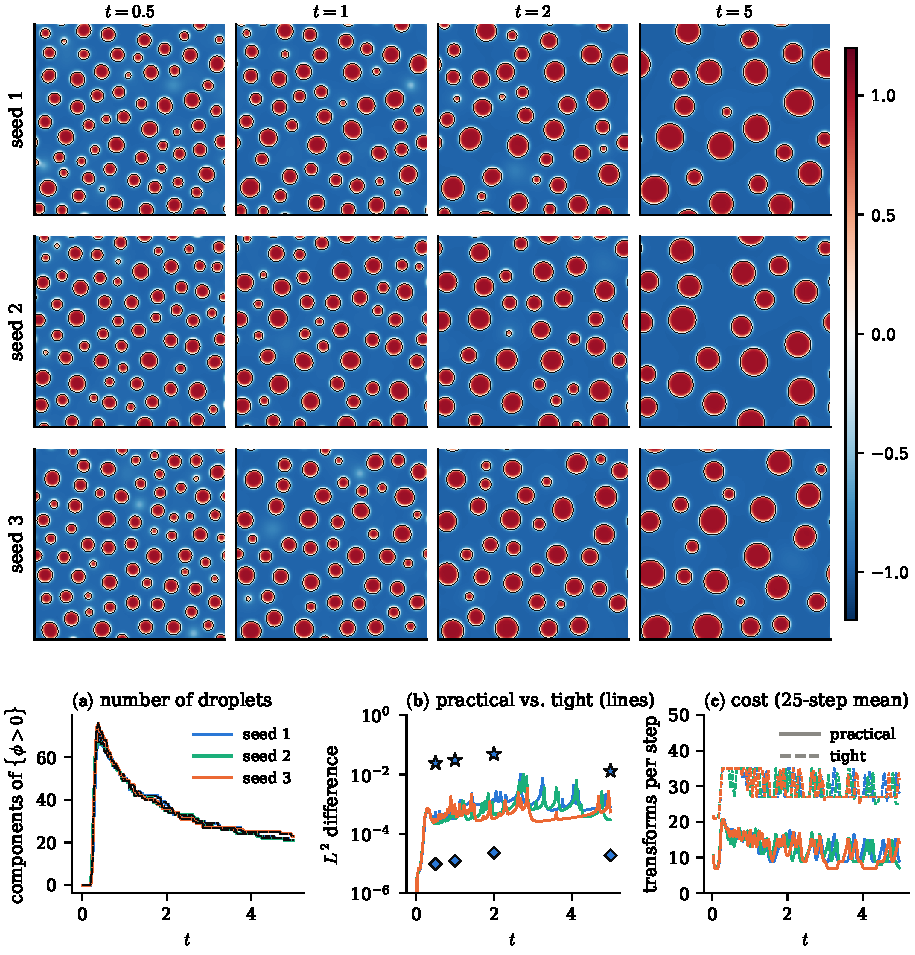
\includegraphics[width=\linewidth]{../figs/figS2_seeds.pdf}
\caption{Nonzero mean ($[0,6.4)^2$, $N=256$, $\eps=0.04$, $A=0$, $\tau=0.002$, $\bar\phi=-0.5$). Top: practical $\phi$ for seeds 1--3 at $t=0.5,1,2,5$, limits $[-1.2,1.2]$ (values in $[-0.980,1.039]$), tight zero level set black. (a)~Components of $\{\phi>0\}$: practical coloured, tight black dashed. (b)~$L^2$ difference practical--tight (lines, colours as in (a)); seed~1, tight: $\tau$ against $\tau/2$ (stars), $N$ against $2N$ (diamonds). (c)~Transforms per step, 25-step moving average: practical solid, tight dashed.}\label{fig:seeds}
\end{figure}

\begin{table}[tbp]
\caption{Seed study (practical Armijo, p, against tight Newton--PCG, t): transforms FFT$_{\rm p}$ / FFT$_{\rm t}$ and the factor FFT$_{\rm t}$/FFT$_{\rm p}$; failures; number of steps (of $2500$) with different droplet counts (largest difference); largest $\delta_\Gamma$ at $t=0.5,1,2,5$; largest $L^2$ difference; largest (T$_E$) ratio; largest mass drift.}\label{tab:seeds}
\centering\scriptsize\setlength{\tabcolsep}{3pt}
\begin{tabular}{lcccccccc}
\toprule
seed & FFT$_{\rm p}$ / FFT$_{\rm t}$ & FFT$_{\rm t}$/FFT$_{\rm p}$ & failures & count differs (max) & $\max_k\delta_\Gamma(t_k)$ & $\max_n\|\phi_p-\phi_t\|$ & (T$_E$) ratio & mass drift\\
\midrule
1 & 31328 / 74300 & 2.37 & 0 & 4 (1) & $1.6\cdot10^{-5}$ & $1.0\cdot10^{-2}$ & $3.1\cdot10^{-4}$ & $4.9\cdot10^{-15}$\\
2 & 31190 / 73616 & 2.36 & 0 & 4 (1) & $1.0\cdot10^{-5}$ & $1.0\cdot10^{-2}$ & $2.9\cdot10^{-4}$ & $2.2\cdot10^{-15}$\\
3 & 30288 / 73752 & 2.44 & 0 & 3 (1) & $1.3\cdot10^{-5}$ & $3.4\cdot10^{-3}$ & $3.3\cdot10^{-4}$ & $6.8\cdot10^{-15}$\\
\bottomrule
\end{tabular}

\end{table}

\emph{Refinement (seed~1 only, tight).} $N=512$: $L^2$ difference $\le2.3\cdot10^{-5}$, $\delta_\Gamma\le5.1\cdot10^{-7}$ at $t=0.5,1,2,5$, same droplet count at every step. $\tau/2$: $L^2$ difference $1.3\cdot10^{-2}$--$4.8\cdot10^{-2}$, $\delta_\Gamma=3.0\cdot10^{-4}$--$5.2\cdot10^{-4}$; counts equal at the output times ($65,50,38,21$) but different at $148$ of $2500$ steps (by up to $4$). Event timing is therefore not converged to one step at $\tau=0.002$.

\emph{Practical versus tight (all seeds; \cref{fig:seeds,tab:seeds}).} No failures (practical $\le9$ iterations, tight $\le4$ Newton iterations, cap $60$); $\Et$ decreases at every step of all six runs; counts rise from $0$ to $67$--$76$ at $t\approx0.35$ and coarsen to $21$--$23$; counts differ at $3$--$4$ of $2500$ steps, by one, against $148$ for $\tau/2$; $\delta_\Gamma\le1.6\cdot10^{-5}$ at the output times ($20$--$63$ times less than the $\tau/2$ effect, seed~1); the largest $L^2$ differences ($1.0\cdot10^{-2}$, $1.0\cdot10^{-2}$, $3.4\cdot10^{-3}$ at $t=2.68,2.75,2.86$) occur at or one step after a droplet removal that happens one step earlier in one run, the median being below $10^{-3}$; $57.6$--$58.9\%$ fewer transforms (practical Armijo against tight Newton--PCG).

\subsection{Synthesis and concluding remarks}\label{sec:conclusion}
\begin{table}[tbp]
\caption{Practical rule with Armijo inner method (p) versus tightly converged Newton--PCG (t) on all lockstep runs: steps, total transforms, saving, topological events (merger or disappearance steps; for the seeds, steps with different droplet counts), largest $L^2$ difference, largest (T$_E$) ratio and mass drift. $\Et$ decreased at every step of every run.}\label{tab:summary}
\centering\scriptsize\setlength{\tabcolsep}{3pt}
\begin{tabular}{lrrrrlccc}
\toprule
run & steps & FFT$_{\rm p}$ & FFT$_{\rm t}$ & fewer & events & $\max_n\nrm{\phi_{\rm p}^n-\phi_{\rm t}^n}$ & (T$_E$) ratio & mass drift\\
\midrule
labyrinth, $512^2$, $\tau=0.004$ & 2500 & 43892 & 112406 & 61.0\% & -- & $4.7\cdot10^{-3}$ & $7.9\cdot10^{-5}$ & $6.0\cdot10^{-15}$\\
merger, $128^2$, $\tau=10^{-3}$ & 500 & 5140 & 11180 & 54.0\% & same & $8.8\cdot10^{-7}$ & $6.3\cdot10^{-6}$ & $1.7\cdot10^{-15}$\\
ripening, $256^2$, $\tau=10^{-3}$ & 2000 & 14492 & 43278 & 66.5\% & same & $4.3\cdot10^{-5}$ & $6.3\cdot10^{-5}$ & $3.7\cdot10^{-15}$\\
$\bar\phi=-0.5$, seed 1, $256^2$, $\tau=0.002$ & 2500 & 31328 & 74300 & 57.8\% & 4/2500 & $1.0\cdot10^{-2}$ & $3.1\cdot10^{-4}$ & $4.9\cdot10^{-15}$\\
$\bar\phi=-0.5$, seed 2, $256^2$, $\tau=0.002$ & 2500 & 31190 & 73616 & 57.6\% & 4/2500 & $1.0\cdot10^{-2}$ & $2.9\cdot10^{-4}$ & $2.2\cdot10^{-15}$\\
$\bar\phi=-0.5$, seed 3, $256^2$, $\tau=0.002$ & 2500 & 30288 & 73752 & 58.9\% & 3/2500 & $3.4\cdot10^{-3}$ & $3.3\cdot10^{-4}$ & $6.8\cdot10^{-15}$\\
\bottomrule
\end{tabular}

\end{table}

\Cref{tab:summary} collects the lockstep comparisons: the practical rule (Armijo) used $54$--$67\%$ fewer transforms than tight Newton--PCG, reproduced merger and disappearance steps, matched droplet radii to $7.4\cdot10^{-5}$ and droplet counts at the output times, and kept $\Et$ decreasing, as \cref{thm:energysafe} guarantees. The unrelaxed iteration diverged in regimes not covered by \cref{cor:linear}, and fixed relaxed sweeps lost order, consistent with \eqref{eq:fixedKres} and \cref{prop:linfixed}; globalized methods stopped by \cref{alg:step} avoided both.

The arguments of \cref{sec:scheme,sec:solver} use only convexity of the implicit part and the constant-coefficient preconditioner, and should extend to other secant and convex-splitting schemes, BDF2 variants and finite-difference discretizations. Error bounds polynomial in $\eps^{-1}$ and logarithmic potentials, where maximum-norm control must be replaced by separation from the singular values, need further ideas.

\medskip{\sloppy\noindent\textbf{Code and data.} The archive \texttt{ch\_inner\_iterations\_submission.zip} contains the solver (\texttt{code/chsolver.py}), the simulation scripts (\texttt{experiments.py}, \texttt{fig\_experiments.py}, \texttt{fig\_experiments2.py}), the raw data (\texttt{data/}), the diagnostics (\texttt{diagnostics.py}, which writes every number quoted in \cref{sec:numerics} to \texttt{data/summary.json}) and the plotting script. From the stored data, all figures and tables are regenerated by \texttt{python3 diagnostics.py} followed by \texttt{python3 make\_figures.py 1 2 3 4 5 6 7 S2 tables}; the commands that rerun each simulation are listed in \texttt{code/README.md}.\par}
